% Native editable composition from verified, unchanged IDE images.
\par
\begin{figure}[htbp]
\centering
\sbox0{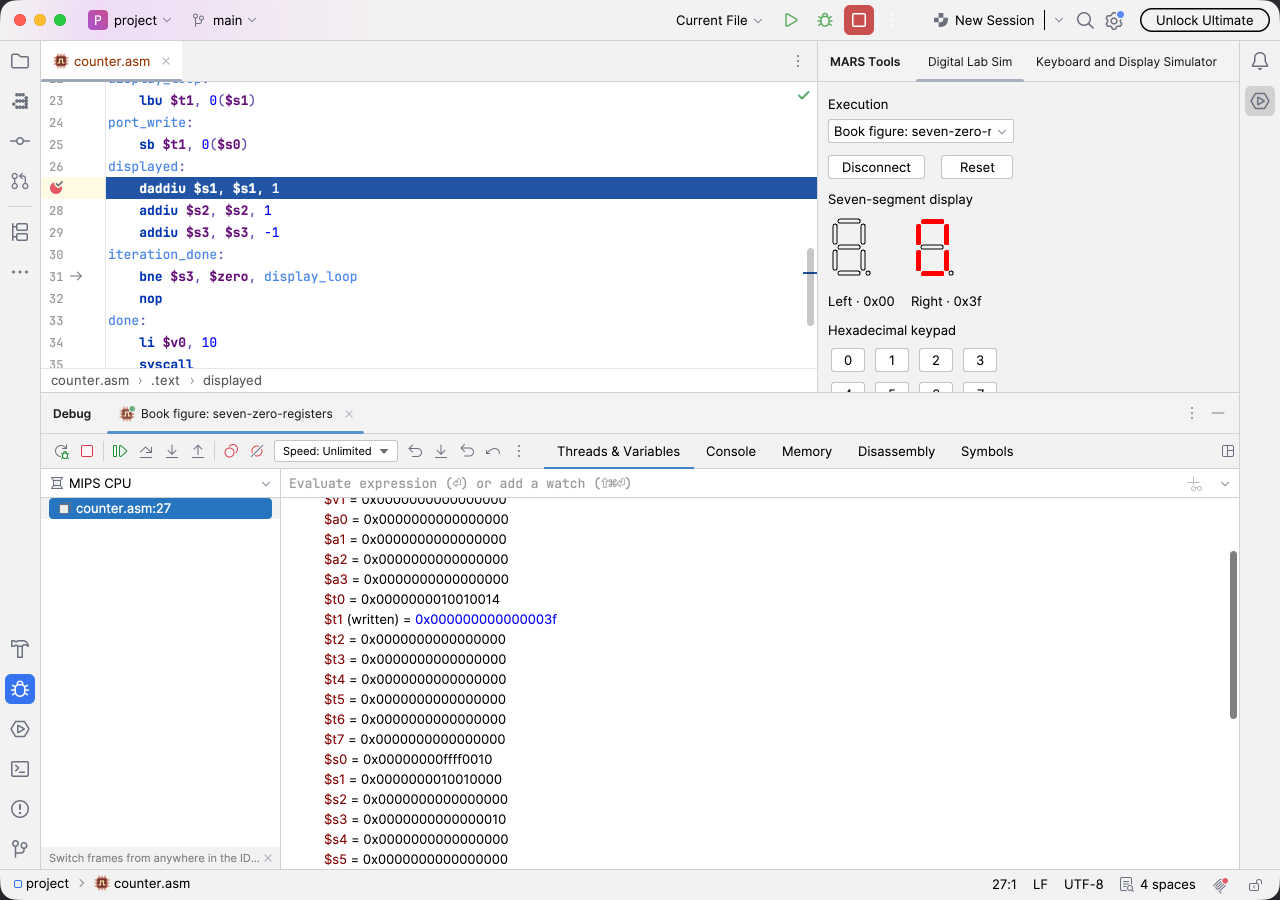
\includegraphics[artifact]{packages/005-seven-segment-counter/captures/f02-zero-glyph/registers.png}}
\sbox2{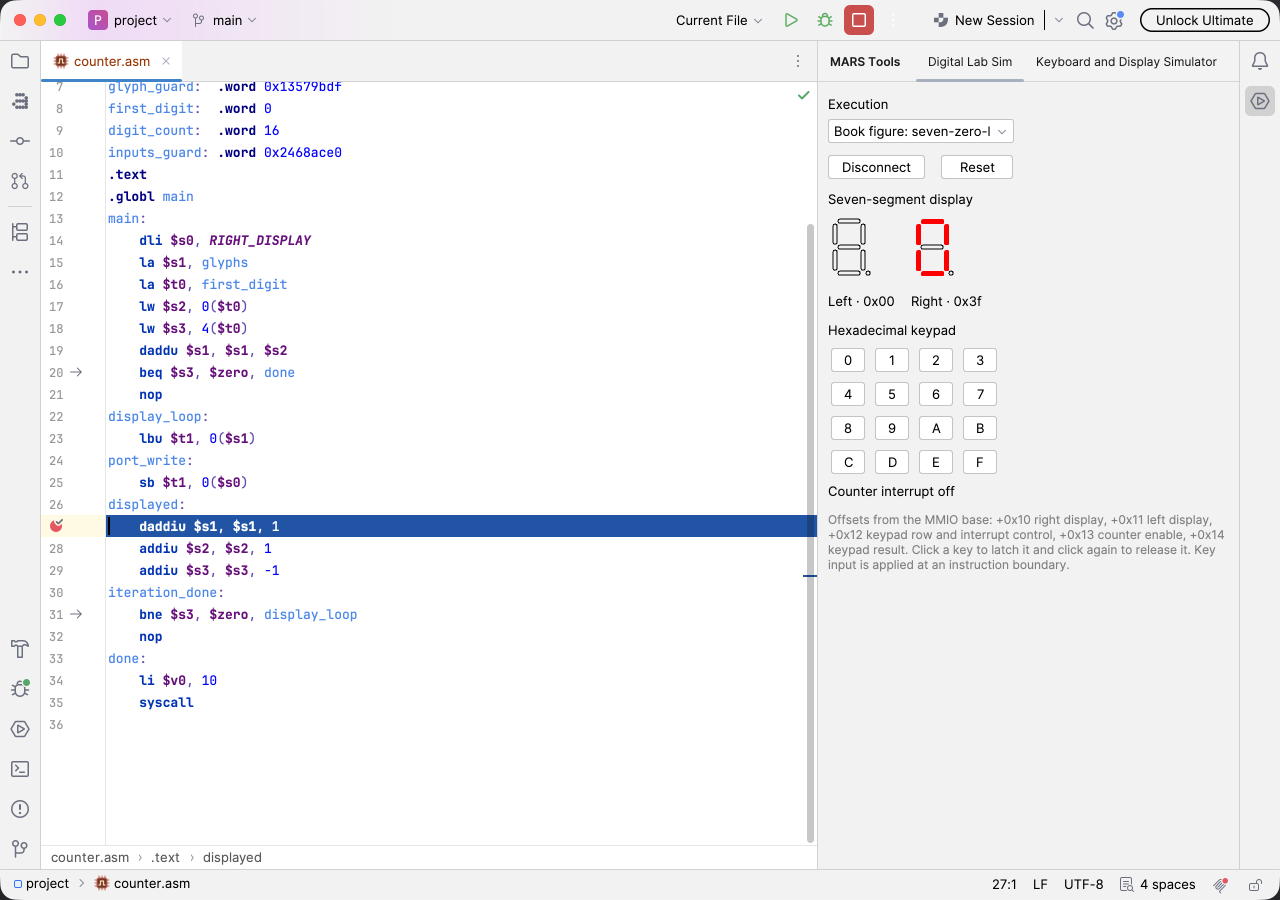
\includegraphics[artifact]{packages/005-seven-segment-counter/captures/f02-zero-glyph/lab.png}}
\edef\MARSzerosourceLeft{\the\dimexpr0.036718750\wd0\relax}
\edef\MARSzerosourceBottom{\the\dimexpr0.774444444\ht0\relax}
\edef\MARSzerosourceRight{\the\dimexpr0.611718750\wd0\relax}
\edef\MARSzerosourceTop{\the\dimexpr0.147777778\ht0\relax}
\edef\MARSzerolabLeft{\the\dimexpr0.643750000\wd2\relax}
\edef\MARSzerolabBottom{\the\dimexpr0.652222222\ht2\relax}
\edef\MARSzerolabRight{\the\dimexpr0.228906250\wd2\relax}
\edef\MARSzerolabTop{\the\dimexpr0.213333333\ht2\relax}
\edef\MARSzeroregistersLeft{\the\dimexpr0.246093750\wd0\relax}
\edef\MARSzeroregistersBottom{\the\dimexpr0.075555556\ht0\relax}
\edef\MARSzeroregistersRight{\the\dimexpr0.597656250\wd0\relax}
\edef\MARSzeroregistersTop{\the\dimexpr0.873333333\ht0\relax}
\begin{tikzpicture}[alt={Three annotated details at the first displayed boundary. The next instruction advances the table pointer by one byte. The left display has mask 00 and remains blank; the right display has mask 3f and shows zero with the decimal point off. Registers s2 and s3 still contain zero and sixteen.}]
\node[anchor=north west,inner sep=0,font=\small\bfseries] (source-title) at (6mm,0) {Stop after the store, before the updates};
\node[anchor=north west,inner sep=0] (source) at ([yshift=-1mm]source-title.south west) {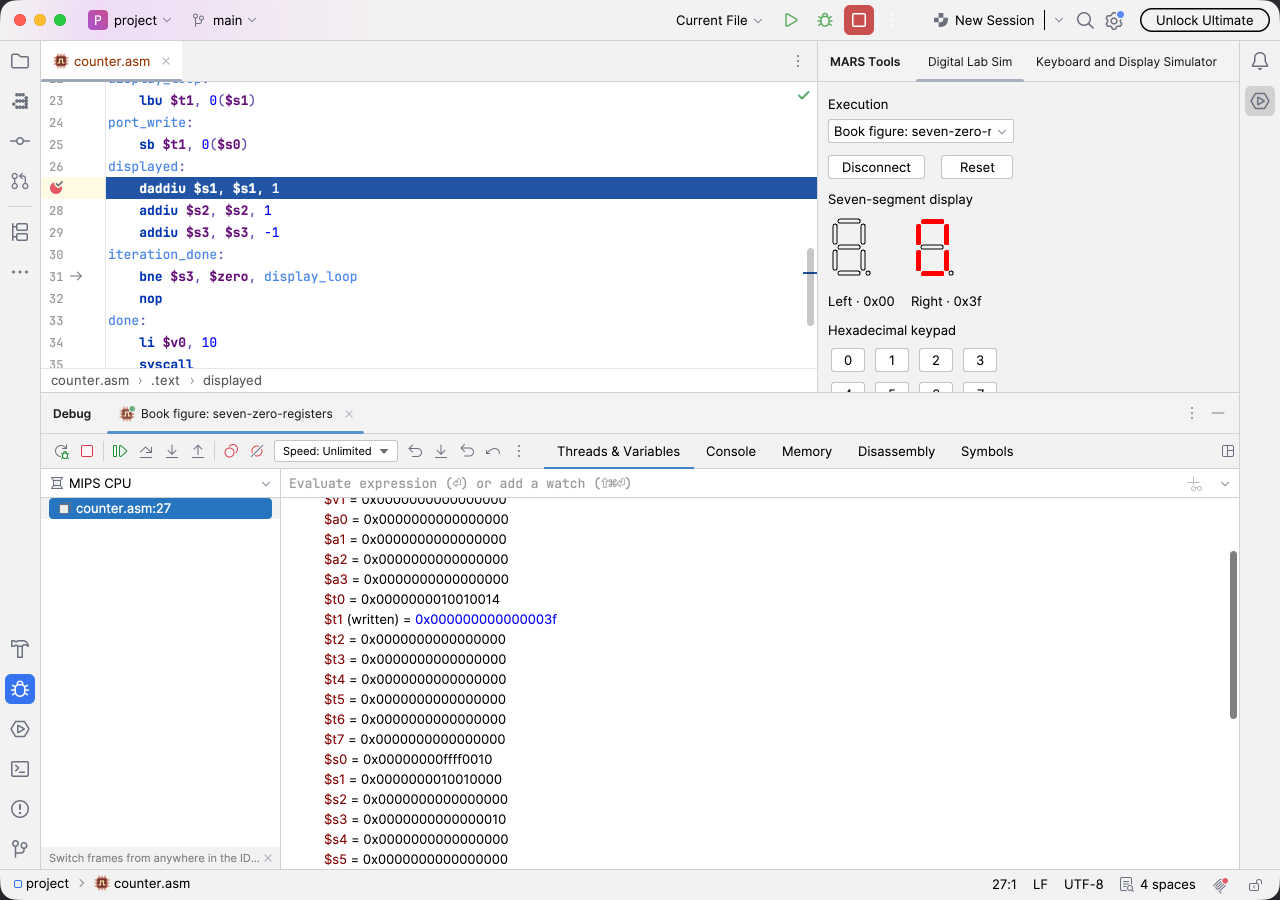
\includegraphics[width=0.7\linewidth,artifact,trim={\MARSzerosourceLeft{} \MARSzerosourceBottom{} \MARSzerosourceRight{} \MARSzerosourceTop{}},clip]{packages/005-seven-segment-counter/captures/f02-zero-glyph/registers.png}};
\begin{scope}[shift={(source.south west)},x={($(source.south east)-(source.south west)$)},y={($(source.north west)-(source.south west)$)}]
\draw[black,line width=0.7pt] (0.135555556,0.057142857) rectangle (0.515555556,0.371428571);
\node[draw=black,fill=white,circle,inner sep=1.5pt,font=\footnotesize] at ($(0.135555556,0.371428571)+(-3mm,0)$) {1};
\end{scope}
\node[anchor=north west,inner sep=0,font=\small\bfseries] (lab-title) at ([yshift=-2mm]source.south west) {A segment mask forms the visible zero};
\node[anchor=north west,inner sep=0] (lab) at ([yshift=-1mm]lab-title.south west) {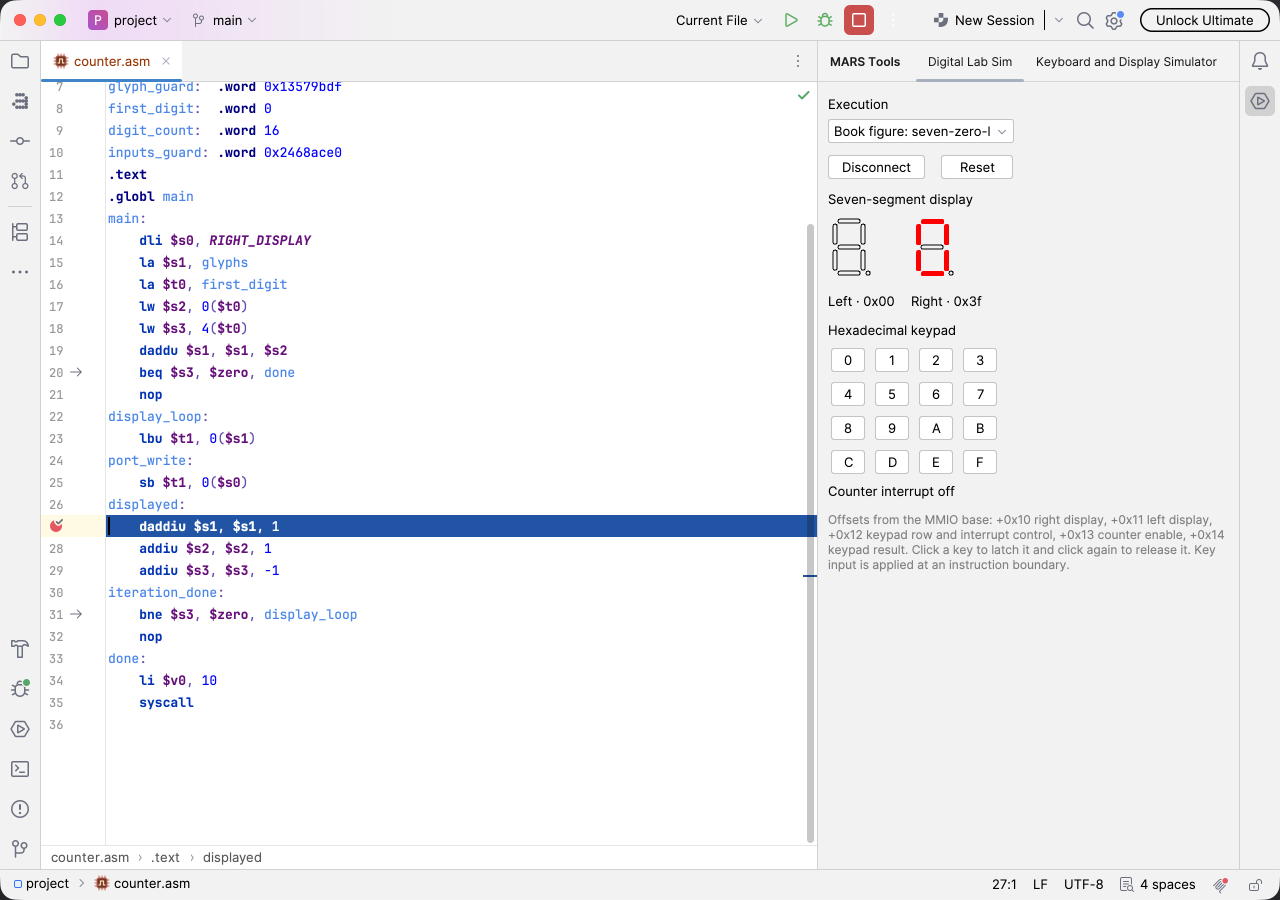
\includegraphics[width=0.34\linewidth,artifact,trim={\MARSzerolabLeft{} \MARSzerolabBottom{} \MARSzerolabRight{} \MARSzerolabTop{}},clip]{packages/005-seven-segment-counter/captures/f02-zero-glyph/lab.png}};
\begin{scope}[shift={(lab.south west)},x={($(lab.south east)-(lab.south west)$)},y={($(lab.north west)-(lab.south west)$)}]
\draw[black,line width=0.7pt] (0.024539877,0.214876033) rectangle (0.815950920,0.818181818);
\node[draw=black,fill=white,circle,inner sep=1.5pt,font=\footnotesize] at ($(0.024539877,0.818181818)+(-3mm,0)$) {2};
\end{scope}
\node[anchor=north west,inner sep=0,font=\small\bfseries] (registers-title) at ([yshift=-2mm]lab.south west) {The counters still describe this iteration};
\node[anchor=north west,inner sep=0] (registers) at ([yshift=-1mm]registers-title.south west) {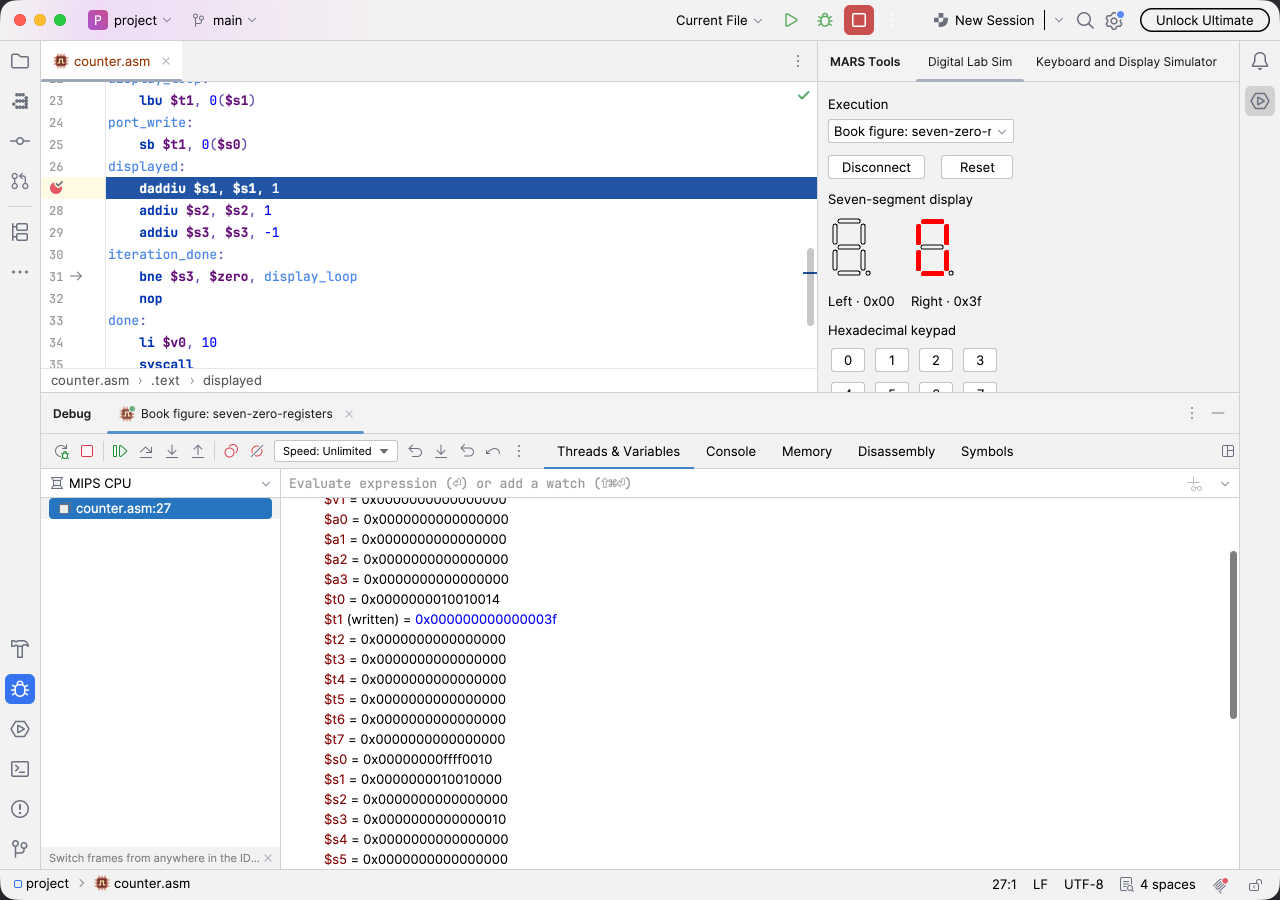
\includegraphics[width=0.43\linewidth,artifact,trim={\MARSzeroregistersLeft{} \MARSzeroregistersBottom{} \MARSzeroregistersRight{} \MARSzeroregistersTop{}},clip]{packages/005-seven-segment-counter/captures/f02-zero-glyph/registers.png}};
\begin{scope}[shift={(registers.south west)},x={($(registers.south east)-(registers.south west)$)},y={($(registers.north west)-(registers.south west)$)}]
\draw[black,line width=0.7pt] (0.030000000,0.065217391) rectangle (0.970000000,0.934782609);
\node[draw=black,fill=white,circle,inner sep=1.5pt,font=\footnotesize] at ($(0.030000000,0.934782609)+(-3mm,0)$) {3};
\end{scope}
\end{tikzpicture}
\par\smallskip
\begin{minipage}{\linewidth}
\small
\begin{enumerate}
\item The blue \texttt{daddiu \$s1, \$s1, 1} is the next instruction. The \texttt{sb} immediately above it has completed. The table pointer still identifies the byte just used; this next instruction will move it to the following table entry.
\item The right mask is \texttt{0x3f}: bits 0 through 5 are set, and the center segment and decimal point are off. The left mask remains \texttt{0x00}. One byte transaction to the fixed right port produces this change; there is no ASCII conversion in the tool.
\item \texttt{\$s2}=0 and \texttt{\$s3}=16 still hold their pre-update values. The index increment and count decrement follow the pointer update. A breakpoint pauses before its highlighted instruction, so the visible zero does not imply that all three loop updates have already happened.
\end{enumerate}
\end{minipage}
\caption{The first byte store forms zero on the right display. The pointer and counter updates have not executed yet.}
\label{capture:005-seven-segment-counter-f02-zero-glyph}
\end{figure}
\par
